\chapter{Introduction}
\label{chap:intro}

\section{Motivation}
\label{chap:motivation}

These days witness the development of information extraction methods, which are fruitfully exploited for automatic construction of Knowledge Graphs (KGs). These are large collections of relational facts in the $\langle subject \rangle \langle predicate \rangle \langle object \rangle$ format. Such triples reflect facts about the real world, which can be converted to facts over unary and binary relations in predicate calculus. Every such triple can be represented as a binary fact \textit{predicate(subject, object)} if \textit{predicate} is not \textit{type} and a unary fact \textit{object(subject)} otherwise. For example, $\langle Brad \rangle \langle livesIn \rangle \langle Berlin \rangle$ can be rewritten as $livesIn(Brad, Berlin)$ while $\langle Mat \rangle \langle type \rangle \langle artist \rangle$ can be converted to $artist(Mat)$. Examples of KGs include YAGO~\cite{ref28}, Wikidata~\footnote{\url{https://www.wikidata.org}}, FreeBase~\footnote{\url{https://developers.google.com/freebase/}}, etc (see Chapter~\ref{chap:relwork} for details).

Unfortunately, KGs are normally incomplete due to automatic construction. Hence, they are processed under the Open World Assumption (OWA) where missing facts can be true or false. Therefore, the \textit{knowledge completion problem} (also known as \textit{link prediction}) plays an important role in improving the quality of KGs. To achieve this, rule learning approaches~\cite{ref39, ref10} are used to create rules which can infer new potentially missing facts. However, the existing methods only pay attention to positive rules, which do not take exceptions (negated atoms) into consideration and may therefore make wrong predictions. For instance, a rule:

\begin{equation}
r1: livesIn(X,Z) \leftarrow isMarriedTo(X,Y), livesIn(Y,Z)
\end{equation}
\label{rule1}

can be discovered from the graph in Figure~\ref{fig1.1} and exploited to predict new facts $livesIn(Alice, Berlin), livesIn(Dave, Chicago)$ and $livesIn(Lucy, Amsterdam)$. However, in reality the first two facts might be incorrect, since $Alice$ and $Dave$ are researchers and the rule $r1$ might have researcher as an exception. Exceptions should be taken into account in rule learning to improve both the rule quality and the quality of facts it produces.

\begin{figure}[t]
\centering
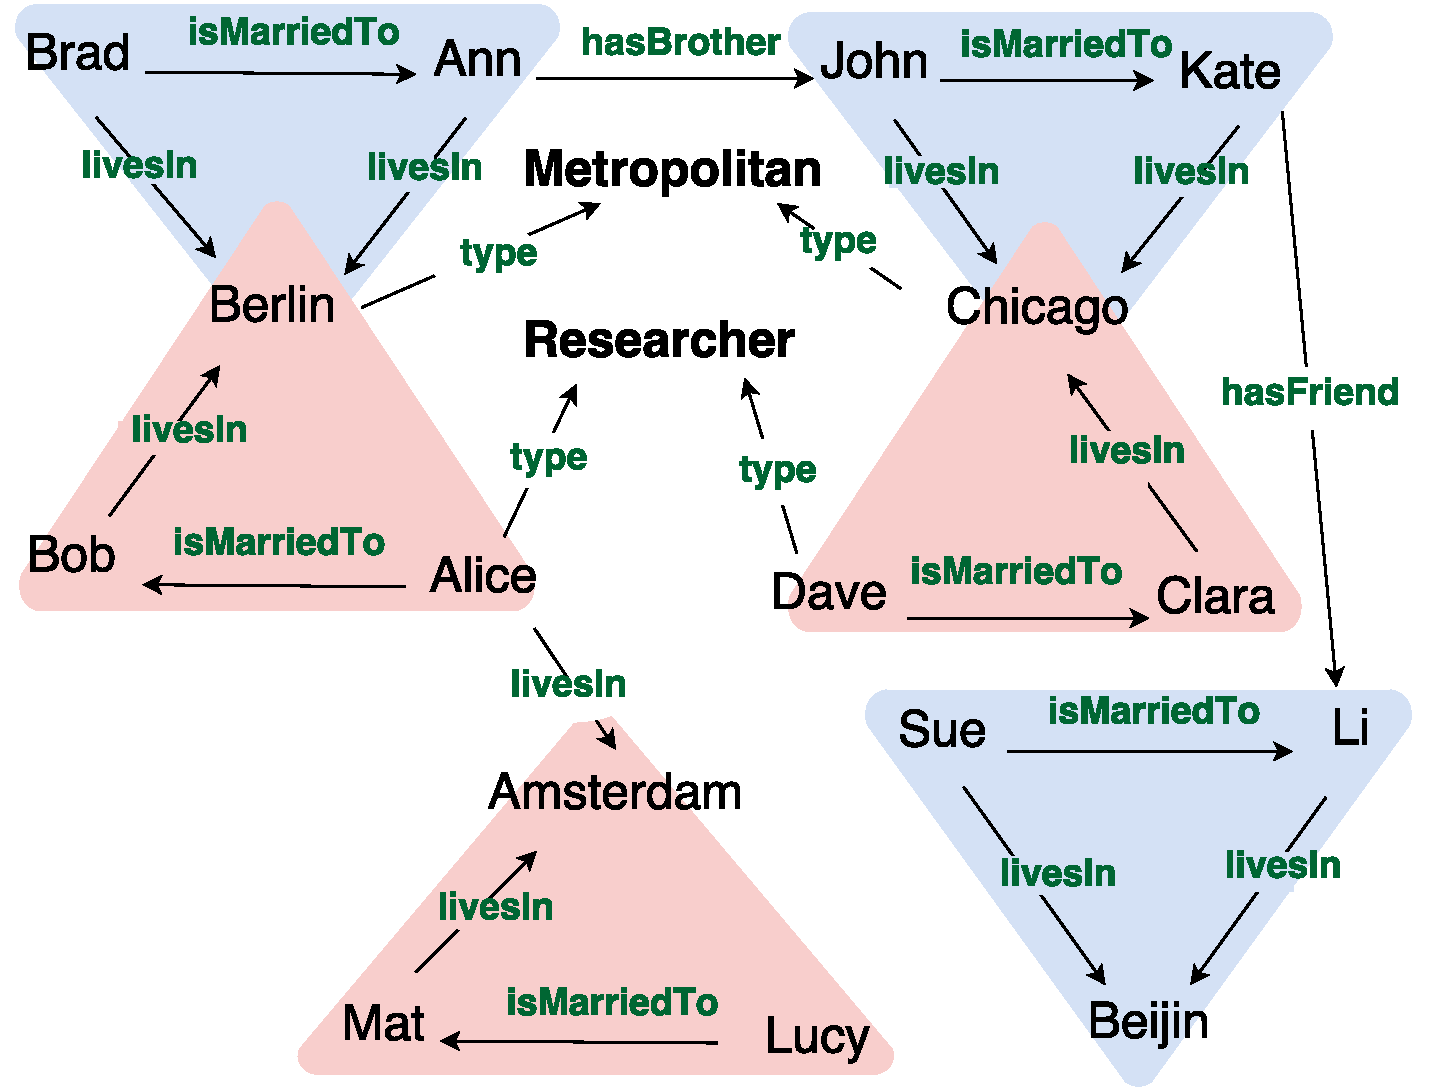
\includegraphics[width=0.75\textwidth]{figures/kg_advanced_col}
\caption{A Visualization of a Knowledge Graph}
\label{fig1.1}
\end{figure}

\section{State of the Art and Its Limitations}

\textit{Nonmonotonic rule learning}~\cite{ref11, ref40, ref41, ref32, ref42} focuses on discovering a set of rules with exceptions (negated atoms) in their bodies (see Chapter \ref{chap:back} for details). However, the state-of-the-art nonmonotonic ILP algorithms cannot be directly applied to our problem due to the following reasons:
\begin{itemize}
\item The \textit{target relations} cannot be explicitly defined because we do not know which parts of the graph need to be extended. A naive solution to this issue is to mine all possible rules for the available predicates in the KG. However, this solution is computationally expensive due to the large number of facts in the original KGs.
\item Second, ILP systems usually exploit positive and \textit{negative examples}. While positive examples are available in our work, negative ones are not given. Besides, the latter are difficult to collect because we cannot differentiate between wrong and unseen triples. Thus, a simple approach to overcome this is to discover rules from solely positive facts.
\item Finally, the \textit{language bias} is not easy to define since the schema of the original data is not given.
\end{itemize}

To overcome the above obstacles, casting our problem into an exploratory data analysis is a suitable solution. The authors in~\cite{ref12} propose association rule mining methods to explore Horn positive rules, and then revise them by inserting exceptions or negated atoms in their bodies to improve the predictive quality of the rules. However, this approach only works on a flattened presentation of a KG, i.e., a collection of unary facts.

\section{Goals}

The aim of this thesis is to:
\begin{itemize}
\item Propose a theory to explore interesting and informative nonmonotonic rules.
\item Build a scalable system in terms of run time to generate rules with exceptions from a large collections of facts.
\item Extensively evaluate the developed system by performing experiments on the real world KGs.
\end{itemize}

\section{Contributions}

This thesis is an extension of the work~\cite{ref12} to handle KGs in their original form. More specifically, we want to mine rules with exceptions from a set of relational facts in KGs treated under the OWA. We transform the knowledge completion problem into \textit{theory revision} task, where given a KG and a set of previously learned Horn rules, the goal is to revise Horn rules to nonmonotonic ones by introducing exceptions. The positive rules can be found by using off-the-shell tools for association rule learning. The revision should be done with the purpose of improving the quality of the revised rules compared to their original versions. To estimate the quality, we exploit the conviction measure~\cite{ref48}.

Our approach consists of four steps. First, for each positive rule, we try to find normal and abnormal sets, that is, set of instances that follow and do not follow a given rule, respectively. Second, we mine exception witness sets, that is, set of unary or binary relations that can eliminate abnormal instances. For instance, \textit{Researcher} is a positive exception for the rule $r1$ based on the KG in Figure~\ref{fig1.1}. Third, we add exceptions to the Horn rules in the form of a single negated atom and define a measure to assess the quality of the obtained revisions. Importantly, the interaction between revised rules is taken into consideration in our approach by a novel concept of \textit{partial materialization}. Finally, exceptions are ranked based on the proposed measures, and the best revision is selected as the final solution. The contributions of this thesis can be summarized as follows:

\begin{itemize}
\item We introduce a framework to revise and improve quality of positive rules by incorporating negated atoms into their bodies.
\item We propose a method for finding exception candidates, assessing their quality and ranking them based on the defined measures. With the novel concept of \textit{partial materialization}, the cross-talk between the rules is taken into account during the revision process.
\item We implement a system that mines Horn rules from a KG and enriches them with exceptions.
\item We construct benchmarks and conduct experiments with YAGO3 and IMDB datasets to test the above-mentioned methodology and the partial materialization concept.
\end{itemize}

\section{Structure}

The outline of this thesis is as follows. Chapter~\ref{chap:relwork} describes related work and presents the literature review. Chapter~\ref{chap:back} provides background and preliminaries for nonmonotonic logic programs and relational association rule learning. Chapter~\ref{chap:frame} presents the rule learning problem that we are tackling and describes our methodology. Chapter~\ref{chap:system} contains the system overview, implementation details and optimization strategies. Chapter~\ref{chap:eval} describes the benchmark construction process, experimental results, their analysis and interpretation. Finally, Chapter~\ref{chap:conclusion} concludes the thesis and outlines approach directions.